\chapter{MARCO TEÓRICO}
%--------------------------2.1-----------------
\section{Unidad de control electrónica ECU}

La \textit{Engine Control Unit} (ECU), o Unidad de Control del Motor, es un módulo electrónico encargado de gestionar el funcionamiento del motor de combustión interna, así como de otros sistemas del vehículo \citep{Bosch_EngineManagement, Heywood2018}. 

En términos simples, la ECU funciona como la “computadora central” del motor y se ve fisicamente como en la Figura \ref{fig:ecu}  recibe señales de sensores, las procesa y emite órdenes a actuadores como inyectores, válvulas de mariposa, sistemas de encendido y ventiladores para mantener el motor funcionando de manera eficiente, segura y dentro de los límites de emisiones permitidos \citep{AcademiaLab_ECU, ClubAuto_ECUfuncionamiento}.

\begin{figure}[h]
	\centering
	
	% 1. El caption automático que ya tiene configurado el estilo APA 7
	\caption{Estructura de la ECU}
	\label{fig:ecu}
	\vspace{0.3cm} % Espacio entre el título y la imagen
	
	% 2. La imagen ajustada
	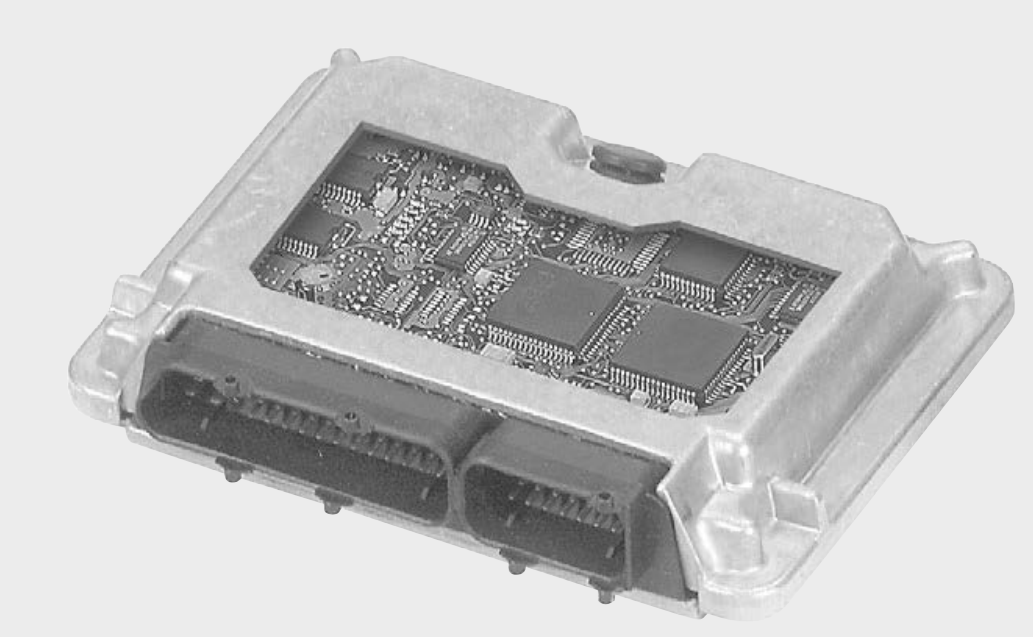
\includegraphics[width=0.75\textwidth]{Images/ECU.png}
	\vspace{0.2cm}
	
	% 3. La nota de fuente formateada según APA 7
	\begin{flushleft}
		\footnotesize \textit{Nota.} Cubierta de la carcasa abierta de una ECU. Fuente: \citep{kaiser2014electronic}.
	\end{flushleft}
\end{figure}

La ECU integra principios de electrónica, control automático y termodinámica del motor, permitiendo regular la mezcla de aire y combustible, el encendido, las emisiones y el consumo energético \citep{Heywood2018, SAE_ECU2015}. Su introducción en los vehículos modernos ha permitido optimizar el rendimiento del motor y cumplir con normas ambientales cada vez más estrictas \citep{SAE_ECU2015}.


Entre las funciones más relevantes de una ECU automotriz se pueden mencionar \citep{Bosch_EngineManagement, ClubAuto_ECUfuncionamiento, Autoavance_ECU2020}:

\begin{itemize}
  \item \textbf{Control de la inyección de combustible}: ajuste de la cantidad, el momento y la duración del chorro de combustible en cada cilindro según la carga del motor, la temperatura del refrigerante, la presión de admisión y otros parámetros.
  \item \textbf{Control del sistema de encendido}: determinación del avance del encendido (ángulo de bujía) para optimizar la combustión de la mezcla aire‑combustible.
  \item \textbf{Control de la admisión de aire}: regulación de la válvula de mariposa, el acelerador electrónico y dispositivos de recirculación de gases (EGR, turbocompresión, etc.) para el caudal de aire al motor.
  \item \textbf{Diagnóstico y monitorización del motor}: detección de anomalías, activación de luces de advertencia en el panel (MIL) y almacenamiento de códigos de falla mediante el sistema OBD‑II.
  \item \textbf{Gestión de otros sistemas}: en vehículos avanzados, la ECU o sus módulos asociados (ECM, PCM, VCM) pueden intervenir en el control de la transmisión automática, el sistema de carga y el aire acondicionado.
\end{itemize}

\subsection{Tipos de modulo de control}
\begin{itemize}
    \item \textbf{ECM} (engine control module), modulo de control del motor.Controla y almacena únicamente los códigos de diagnóstico de fallas (DTCs) de los componentes del motor.
    \item \textbf{PCM} (train power control module), modulo de control del tren de potencia. Controla y almacena datos del motor y la transmisión.
    \item \textbf{VCM} (vehicle control module), modulo de control del vehículo. Controla y almacena datos del motor, la transmisión y otros sistemas del vehículo como sistemas de frenos ABS.\citep{poudel2018design}
\end{itemize}

\subsection{Estructura interna de la ECU} % (microprocesador, memoria, entradas/salidas)
La estructura interna de una ECU se basa en un sistema de hardware y software integrado, donde el núcleo principal es un microcontrolador (CPU) encargado de procesar en tiempo real las señales provenientes de sensores y emitir órdenes a los actuadores del motor \citep{Bosch_EngineManagement, Heywood2018}. Alrededor de este microcontrolador se disponen memorias de tipo flash y ROM, que almacenan el firmware y los mapas de encendido e inyección, así como memoria RAM utilizada para cálculos y variables de estado durante el funcionamiento \citep{Wikipedia_ECU, ClubAuto_ECUfuncionamiento}. 

Además, la ECU integra módulos de acondicionamiento de señales de entrada (filtros, amplificadores y convertidores analógico‑digital) y etapas de potencia de salida (drivers de transistores o MOSFET) para activar correctamente actuadores como inyectores de combustible, válvulas solenoides y ventiladores de refrigeración \citep{Autoavance_ECU2020}.
Y se divide en los siguientes sistemas.

\begin{itemize}
    \item \textbf{Periferia} Consta de elementos pasivos resistencias, capacitores. 
    \item \textbf{Circuitos de filtrado} Filtros pasa bajos para contrarrestar ruido y mejorar la señal. 
    \item \textbf{Fuente} Elementos pasivos y semiconductores resistencias, capacitores, diodos y reguladores de tensión. 
    \item \textbf{Procesamiento de datos} Usa 2 sistemas clave, la memoria la que almacena todos los datos, y el procesador que lee todos los datos. 
    \item \textbf{Driver} Maneja todos los actuadores: transistores, drivers para motores de paso. 
    \item \textbf{Multiplexor} Comparte datos con otras ECUS. 
\end{itemize}

Todos los sistemas mencionados se muestran en conjunto en la Figura \ref{fig:a_ecu}

\begin{figure}[h]
	\centering
	
	% 1. El caption automático con estilo APA 7 (Título arriba)
	\caption{Arquitectura interna de la ECU}
	\label{fig:a_ecu}
	\vspace{0.3cm}
	
	% 2. La imagen
	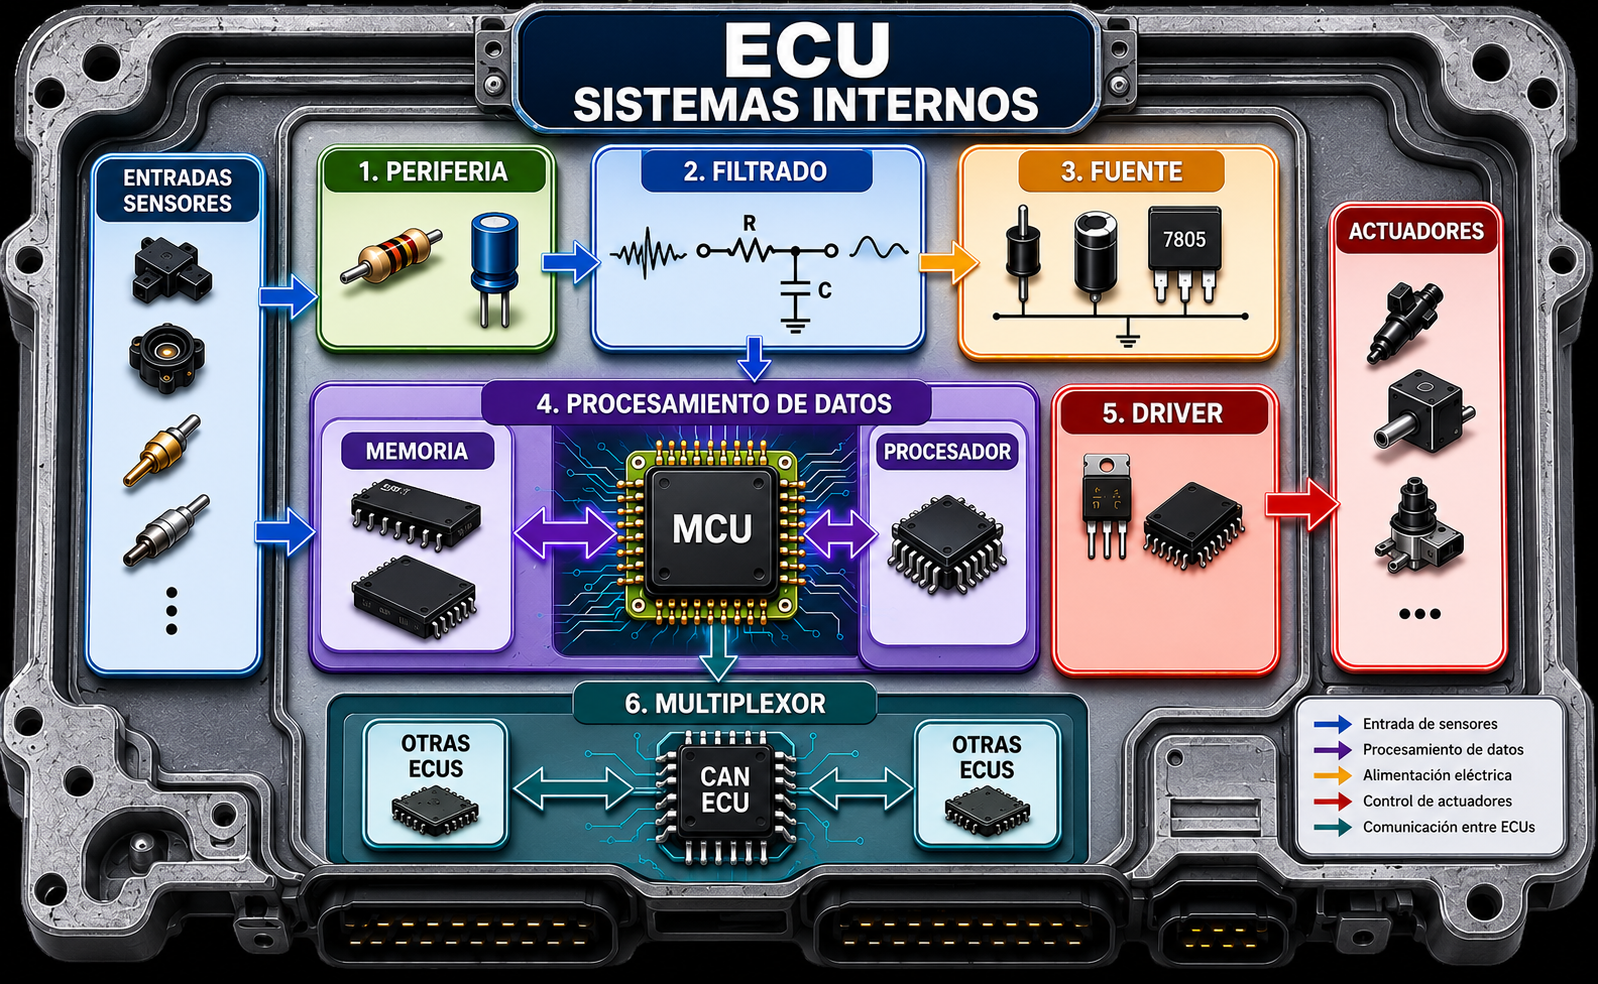
\includegraphics[width=0.9\textwidth]{Images/ESTRUCTURA.png}
	\vspace{0.2cm}
	
	% 3. La nota de fuente formateada según APA 7
	\begin{flushleft}
		\footnotesize \textit{Nota.} Arquitectura interna y conjunto de sistemas dentro de la unidad de control. Elaboración propia basada en \citep{poudel2018design} y generada con apoyo de inteligencia artificial (Gemini).
	\end{flushleft}
\end{figure}

\subsubsection{Procesamiento de señales} % (cómo la ECU interpreta datos)
Para que el microprocesador pueda interpretar las señales de los sensores (señales de entrada), estas deben ser convertidas en el módulo de control electrónico de analógicas a digitales. Estas señales luego son acompañadas con los parámetros lógicos grabados en la memoria y luego será elaborada la orden o señales de salida a los actuadores. 

Se muestra un diagrama general del procesamiento de la ECU en la Figura \ref{fig:dia_pro}.

\begin{figure}[h]
	\centering
	
	% 1. El caption automático estilo APA 7 (Título arriba)
	\caption{Diagrama de procesamiento de la ECU}
	\label{fig:dia_pro}
	\vspace{0.3cm}
	
	% 2. La imagen
	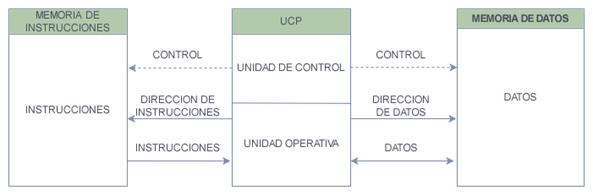
\includegraphics[width=0.8\textwidth]{Images/DIAGRAM.png}
	\vspace{0.2cm}
	
	% 3. La nota de la figura según APA 7
	\begin{flushleft}
		\footnotesize \textit{Nota.} Secuencia lógica de las etapas de entrada, procesamiento y salida de datos en la unidad de control. Elaboración propia.
	\end{flushleft}
\end{figure}

\subsubsection{Parámetros de control del motor} % (mezcla aire-combustible, avance de encendido)
Es necesario diferenciar bien cada una de las fases que esta debe realizar para enviar señales a los diferentes actuadores del vehículo.\\
Para ello se divide el estudio en cuatro bloques de funcionamiento. 
\begin{itemize}
    \item \textbf{Bloque de entrada} Se denomina bloque de entrada a todos los circuitos que se encuentran como receptores de las diferentes señales que van a ingresar a la ECU y antes de que lleguen al microprocesador. Encontramos en este sentido, filtros, amplificadores, conformadores de impulsos, conversores análogos a digital. 
    \begin{itemize}
        \item Regulador de tensión.- El regulador de tensión (5V) es utilizado como señal de entrada para casitodos los sensores de inyección y para la operación interna de memorias y el microprocesador del módulo de control electrónico.
        La tensión regulada es mantenida a pesar de las variaciones de tensión de la batería en 5V ± 15%
        \item Filtrado de señales.-  Los filtros digitales tienen como entrada una señal analógica o digital y en su salida tienen otra señal analógica o digital, pudiendo haber cambiado en amplitud, frecuencia o fase dependiendo de las características del filtro digital. 
        \item Conformadores de impulso.- Actúa para recibir los impulsos de tensión de los órganos de información del encendido. Estos impulsos son modificados en magnitud y en forma, para dejarlos en condiciones que puedan ser procesados por el micro-ordenador. 
        \item Convertidor Análogo – Digital.- La señal que recibe el módulo de control electrónico desde los sensores, no puede ser interpretada por el microprocesador, por lo tanto las señales de los sensores que son análogas, deben ser convertidas a digitales.\\
        Para esta conversión se utilizan transistores de saturación o corte, que se comportan exactamente igual a un relé activado-desactivado. 
    \end{itemize}
    \item \textbf{Bloque de procesamiento} Son todos los circuitos que desarrolla las funciones programadas y que están constituidos circuitalmente por el procesador, memorias y todo circuito que se vea involucrado en la ejecución del software. 
    \begin{itemize}
        \item \textbf{Memorias.-} Es esta se realizan los cálculos matemáticos de acuerdo a las señales de entrada; la memoria se borra cuando se apaga el motor. 
        \begin{itemize}
            \item \textbf{Memoria RAM (Random Access Memory):} El microprocesador utiliza la memoria RAM para saber el estado general y las condiciones del motor y en función a esto hacer funcionar los actuadores. 
            \item \textbf{Memoria KAM (Keep Alive Memory):} La memoria KAM vive con la memoria RAM y su función es de guardar los datos que no se pueden perder al cerrar el contacto, como por ejemplo códigos de fallas aleatorias de sensores.
            
            A diferencia de la memoria RAM, la KAM no se borra al cerrar el contacto, pero si se borra al desconectar la batería.
            
            Cuando en la memoria KAM se almacena un defecto, este permanecerá instalado aun después de ser corregido, debiendo desconectar la batería para que se borre o en algunos casos, se debe proceder al borrado con un scanner. 
            \item \textbf{Memoria EPROM (Erasable Programmable Read Only Memory):} En la memoria EPROM (programable) o PROM (programada) es donde el microprocesador consulta todas las calibraciones del vehículo, tales como el peso del mismo y la compresión del motor. Al cerrar el contacto o desconectar la batería, esta memoria no se borra. 
            \item \textbf{Memoria ROM (Read Only Memory):} Esta memoria mantiene grabados los programas con todos los datos, curvas características y valores teóricos con los que ha de funcionar el sistema.
            
            Esta memoria es utilizada por el microprocesador para comparar los parámetro de cada sensor en cada situación y en los casos en que el microprocesador detecte alguna anomalía en alguna señal, la reemplazará por un valor de la memoria ROM.
            
            La memoria ROM es una memoria de consulta y al igual que la memoria EPROM no se borra ni al cerrar el contacto, ni al desconectar la batería.
        \end{itemize}
        \item \textbf{Microprocesador:} Es el componente físico principal dentro de la unidad de control, encargado de ejecutar las instrucciones de software para optimizar el funcionamiento del motor. Este elemento realiza los cálculos matemáticos, la toma de decisiones y ejecuta las estrategias de emergencia.
        Contiene en su interior tres dispositivos fundamentales:
        \begin{itemize}
            \item \textbf{Unidad lógica de calculo (ALU):}Realiza las operaciones aritméticas y las operaciones lógicas.
            \item \textbf{Acumulador:} Es una memoria intermedia que permite al CPU guardar datos mientras trabaja con otros que están directamente relacionados con el proceso en curso.
            \item \textbf{Unidad de control:} Es el elemento activo que solicita los datos, controla las entradas, las salidas y el desarrollo de las operaciones.
        \end{itemize}
        
    \end{itemize}

    \item \textbf{Bloque de salida} Así como las señales son tratadas al ingresar, existen circuitos que se encuentran entre las salidas del microprocesador y los diferentes elementos que van a ser actuados como por ejemplo: bobinas de encendido, inyectores, relés, etc. \\
    Tenemos los siguientes componentes importantes en este bloque:
    \begin{itemize}
        \item Convertidor digital - análogo.- Así como las señales de los sensores deben ser transformadas en digitales, para que puedan ser interpretadas por el microprocesador y de esta forma “saber lo que está pasando La señal digital debe convertirse en analógica para controlar los actuadores(señales analógicas).
        
        De esta forma es que todas las señales micro procesadas son convertidas de digitales en análogas para controlar a los actuadores. El convertidor digital recibe un número de 8 BITS y la trasforma en una tensión continua de un valor proporcional al número digital.
        \item Drivers (Controlador de dispositivo).- El drivers están básicamente diseñado para controlar los actuadores, como por ejemplo los inyectores, bobinas, relés, entre otros, estos circuitos deben cumplir con requisitos de manejo de potencia puesto que la corriente que se maneja en muchos de ellos alcanza los 5A y los voltajes operados pueden llegar a picos de hasta 400V.
        \begin{itemize}
            \item Transistores
            \item Circuitos integrados de control
        \end{itemize}
        \item Circuitos de potencia con transistores.- Se encargan de dar los pulsos de activación a las bobinas de encendido, inyectores, relés, etc. para de esta manera poner en funcionamiento a cada uno de los actuadores. 
        
   \end{itemize}
    \item \textbf{Bloque de soporte}  Se denomina así al conjunto de componentes que tienen como función alimentar a los circuitos internos mencionados anteriormente. Lo constituye la fuente de alimentación de la ECU.
    \begin{itemize}
        \item Regulador de voltaje.-
        \item Fuente de alimentación de la ECU.- Los ECM disponen de una fuente de poder interna que proporciona distintos tipos de voltajes para energizar componentes como sensores y Actuadores. Estos voltajes pueden tener una variación.\\Conformados por:
        \begin{itemize}
            \item Diodos rectificadores y zener.
            \item Condensadores.
            \item Reguladores de Tensión.
            \item Resistencias.
        \end{itemize}
    \end{itemize}
    Datos importante de la parte de bloque de soporte:
    \begin{itemize}
        \item + 5 volt. + - 0.5 V voltaje de suministro para sensores análogos.
        \item + 8 volt. + - 0.5 V voltaje de suministro para sensores digitales o PWM.
        \item + 12,5 volt. + - 1V voltaje de suministro para sensores de frecuencia electrónicos.
        \item + 105 volt. + - 0.5 voltaje de suministro para solenoides para inyección de combustible.
    \end{itemize}
    Para el negativo, existen tres posibilidades de masas en una ECU, estas son: 
    \begin{itemize}
        \item \textbf{Masa digital:} Usada por la ECU para el sistema de procesamiento de datos, Procesador y Memoria.
        \item \textbf{Masa análoga:} Usada por la ECU para circuitos análogos, por ejemplo conversores análogos a digital.
        \item \textbf{Masa de potencia:} Usada por la ECU para circuitos de fuente y control de actuadores principalmente ej. , regulador de tensión y principalmente transistores.
        \item \textbf{Masa de blindaje:} La Ecu posee un circuito de blindaje, el cual es capaz de transportar las señales dentro de la ECU sin la presencia de ruido electromagnético.
    \end{itemize}
\end{itemize}

Se presenta un resumen en la Figura \ref{fig:esquema_ecu}

\begin{figure}[h]
	\centering
	
	% 1. El caption automático estilo APA 7 (Título arriba)
	\caption{Esquema de la unidad de control electrónica ECU}
	\label{fig:esquema_ecu}
	\vspace{0.3cm}
	
	% 2. La imagen ajustada al ancho del texto para evitar Overfull \hbox
	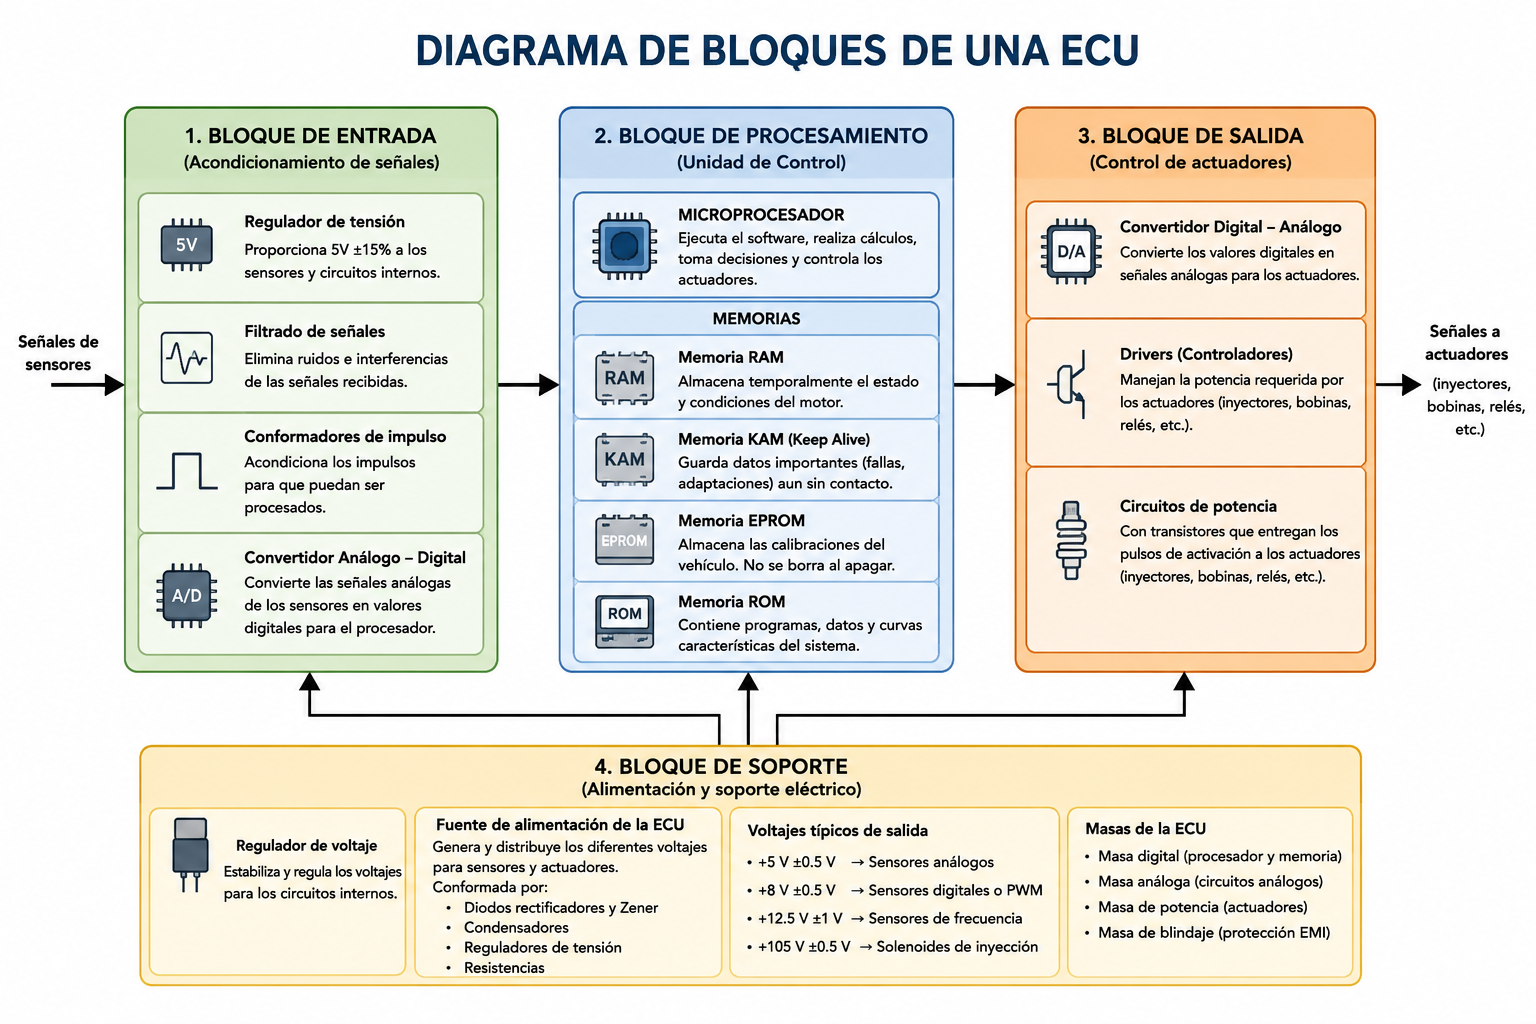
\includegraphics[width=1.0\textwidth]{Images/ChatGPT.png}
	\vspace{0.2cm}
	
	% 3. La nota de la figura según APA 7
	\begin{flushleft}
		\footnotesize \textit{Nota.} Diagrama esquemático integral de los bloques funcionales de la unidad de control. Elaboración propia, generada con apoyo de inteligencia artificial (Gemini).
	\end{flushleft}
\end{figure}

\subsection{Importancia de la ECU en el consumo de combustible}
La ECU desempeña un papel fundamental en la optimización del consumo de combustible, actúando como el elemento central que regula la mezcla aire‑combustible, el encendido, la admisión de aire y la gestión general del motor \citep{Bosch_EngineManagement, Heywood2018}. Mediante el uso continuo de sensores de presión de admisión, temperatura, posición del acelerador, velocidad y carga, la ECU ajusta en tiempo real la cantidad de combustible inyectado, el avance del encendido y el flujo de aire, favoreciendo siempre una combustión lo más completa y eficiente posible \citep{SAE_ECU2015, ClubAuto_ECUfuncionamiento}.

Esta regulación permanente permite que el motor funcione cerca de su punto óptimo de eficiencia en una amplia gama de condiciones de conducción, lo que se traduce en una reducción del consumo específico de combustible y en menores emisiones contaminantes \citep{AcademiaLab_ECU, CentralitaBSI_EficienciaCombustible}. 

Además, en vehículos con transmisión automática, la ECU colabora con otros módulos de control (por ejemplo, ECU de transmisión) para seleccionar el momento más adecuado para cambiar de marcha, lo que contribuye a mantener el motor en rangos de revoluciones donde el consumo de combustible es más bajo \citep{SAE_ECU2015, PedalCommander_ECUtuning}.

Por lo tanto la cantidad de combustible a inyectar es determinado teniendo en cuenta también la cartografía de inyección que esta memorizada en la unidad de control y que intenta en todo momento evitar la emisión de contaminantes (humo negro) ver Figura \ref{fig:carto}. Si el volumen de aire aspirado es demasiado bajo la cantidad de combustible inyectado es limitado a un valor que no provoque humos negros.

\begin{figure}[h]
	\centering
	
	% 1. El caption automático estilo APA 7 (Título arriba)
	\caption{Cartografía de inyección}
	\label{fig:carto}
	\vspace{0.3cm}
	
	% 2. La imagen ajustada para una mejor visualización de los datos
	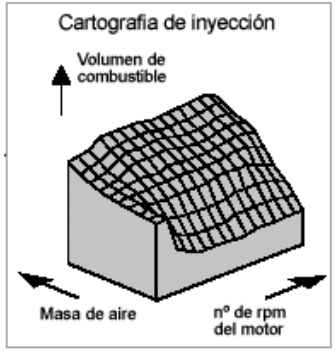
\includegraphics[width=0.5\textwidth]{Images/Conbu.png}
	\vspace{0.2cm}
	
	% 3. La nota de la figura según APA 7
	\begin{flushleft}
		\footnotesize \textit{Nota.} Mapa tridimensional de calibración que relaciona la carga del motor y las revoluciones por minuto para determinar el tiempo de inyección. Tomado de \citep{poudel2018design}.
	\end{flushleft}
\end{figure}

La unidad de control tiene memorizado un mapa de comienzo de la inyección.Este mapa toma como referencia principal el nº de rpm del motor y la cantidad de combustible inyectado ver Figura \ref{fig:rela} Como parámetro corrector se utiliza la temperatura del motor que actúa también sobre el comienzo de la inyección.

\begin{figure}[h]
	\centering
	
	% 1. El caption automático estilo APA 7 (Título conciso arriba)
	\caption{Relación de inyección entre el sensor MAP y las RPM}
	\label{fig:rela}
	\vspace{0.3cm}
	
	% 2. La imagen con su escala original
	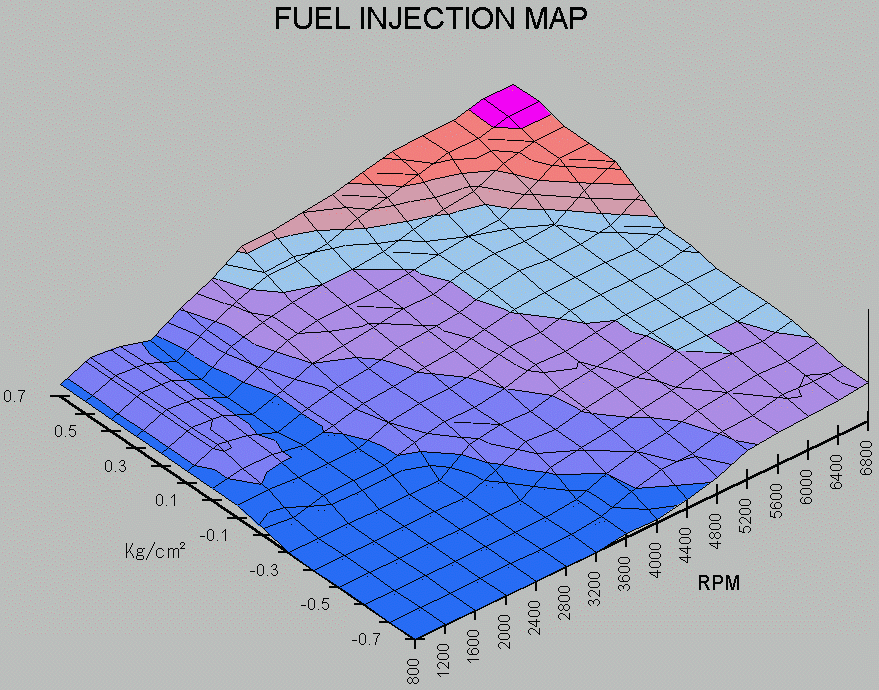
\includegraphics[width=0.63\textwidth]{Images/mAP2.png}
	\vspace{0.2cm}
	
	% 3. La nota de la figura según APA 7 (Con los detalles específicos)
	\begin{flushleft}
		\footnotesize \textit{Nota.} Comportamiento de la dosificación de combustible en un motor de cuatro tiempos operando a nivel del mar en función de la presión absoluta del colector y el régimen de giro. Tomado de \citep{ForoClubJapo_ECU}.
	\end{flushleft}
\end{figure}

En resumen, la ECU no solo mejora el rendimiento y la respuesta del motor, sino que es un componente clave para lograr una \textbf{operación económica y sostenible} del vehículo, incrementando la eficiencia del combustible sin comprometer significativamente la potencia entregada \citep{Bosch_EngineManagement, SERNAUTO_ECUeficiencia}.

%-------------------------2.2-----------------
\section{Protocolos de comunicación en vehículos}

En los vehículos modernos, la comunicación entre unidades de control electrónico (ECU) se realiza a través de diversos buses de datos en serie, que permiten integrar sistemas de motor, transmisión, chasis, seguridad y entretenimiento en una red coherente \citep{Navixy_AutomotiveBuses, MSG_CommunicationBuses}. Entre los protocolos más utilizados se encuentran CAN, LIN, FlexRay y MOST, cada uno con características distintas de velocidad, ancho de banda, costo y aplicación específica \citep{ProtocolosComunicacionAutomotriz}.

\subsection{CAN}

El protocolo \textit{Controller Area Network} (CAN) es el estándar más extendido en la comunicación interna de vehículos, utilizado para conectar unidades de control del motor (ECM), de transmisión (TCM) y sistemas de frenado (ABS), entre otros \citep{Navixy_AutomotiveBuses}. CAN opera sobre un bus de dos hilos (CAN high y CAN low) y permite la transmisión de mensajes priorizados, lo que garantiza que los datos de seguridad y dinámica del vehículo tengan mayor prioridad que los de confort o información \citep{ProtocolosComunicacionAutomotriz}. Su velocidad típica varía desde 125 kbit/s hasta 1 Mbit/s, convirtiéndolo en una solución robusta, económica y tolerante a fallos \citep{MSG_CommunicationBuses}.

\subsection{LIN}

El bus \textit{Local Interconnect Network} (LIN) es un protocolo de baja velocidad diseñado principalmente para aplicaciones de confort y comodidades, como ventanas eléctricas, espejos, luces interiores y sensores de climatización \citep{ProtocolosComunicacionAutomotriz}. Comparado con CAN, LIN es más simple y barato, ya que trabaja con un solo maestro y varios esclavos en topología maestro‑esclavo \citep{MSG_CommunicationBuses}. Aunque su velocidad máxima suele estar alrededor de 20 kbit/s, LIN es ideal para tareas poco críticas donde la prioridad es reducir costos de cableado y electrónica \citep{ProtocolosComunicacionAutomotriz}.

\subsection{FlexRay}

El protocolo FlexRay es un bus de alta velocidad y baja latencia orientado a aplicaciones críticas, como sistemas de conducción avanzada, control de chasis y vehículos autónomos \citep{Navixy_AutomotiveBuses, Autoavance_FlexRay}. FlexRay ofrece tiempos de respuesta deterministas y soporta tasas de transferencia de hasta 10 Mbit/s, lo que permite manejar grandes volúmenes de datos en tiempo real \citep{MSG_CommunicationBuses}. Además, su topología dual‑canal permite redundancia y alta disponibilidad, características clave para funciones de seguridad que no admiten interrupciones \citep{Autoavance_FlexRay}.

\subsection{MOST}

El bus MOST (\textit{Media Oriented Systems Transport}) está dedicado a la transmisión de datos multimedia, como audio, video y señales de info‑entretenimiento, dentro del vehículo \citep{Navixy_AutomotiveBuses}. MOST utiliza un anillo óptico o eléctrico y soporta velocidades de 25, 50 o 150 Mbit/s, permitiendo integrar pantallas, sistemas de navegación, reproductores de audio y dispositivos de comunicación sin afectar las redes de control principal \citep{ProtocolosComunicacionAutomotriz}. Su diseño está orientado a mantener alta calidad de señal y bajo retardo en el transporte de flujos multimedios, separando esta red de la red de control motor‑tracción construida sobre CAN o FlexRay \citep{ProtocolosComunicacionAutomotriz}.

El resumen de lo abordado se presenta en la Tabla \ref{table:caract}


\begin{table}[htbp]
	\centering
	% Título separado bajo norma estricta APA 7
	\captionsetup{labelformat=simple, labelsep=newline, textfont=it, labelfont=bf}
	\caption{Comparación de los protocolos de comunicación en vehículos}
	\label{table:caract}
	\vspace{0.3cm}
	
	\begin{tabularx}{\linewidth}{p{2.4cm} X X X X}
		\toprule 
		\rowcolor[rgb]{0.851, 0.851, 0.851}
		\textbf{Ítem} & \textbf{CAN} & \textbf{LIN} & \textbf{FlexRay} & \textbf{MOST} \\
		\midrule 
		Velocidad típica & 125 kbit/s a 1 Mbit/s & Hasta 20 kbit/s & Hasta 10 Mbit/s & 25, 50 o 150 Mbit/s \\
		Aplicación & Control de motor, transmisión, ABS & Comodidades (ventanas, espejos, luces) & Sistemas de seguridad y conducción avanzada & Multimedia (audio, video, infoentretenimiento) \\
		Topología & Bus multidifusión robusto & Maestro-esclavo, sencillo & Dual-canal redundante & Anillo óptico o eléctrico \\
		Prioridad & Alta, con priorización de datos críticos & Baja, tareas no críticas & Alta, determinista & Media, orientado a multimedia \\
		Costo & Moderado & Bajo & Alto & Alto \\
		Latencia & Media & Alta & Muy baja & Media \\
		\bottomrule 
	\end{tabularx}
	\vspace{0.2cm}
	
	\begin{flushleft}
		\footnotesize \textit{Nota.} Elaboración propia.
	\end{flushleft}
\end{table}


%-------------------------2.3----------------
\section{Sistema OBD-II}
\subsection{Evolución del diagnóstico a bordo}

El diagnóstico a bordo, conocido como OBD (\textit{On-Board Diagnostics}), evolucionó desde sistemas muy básicos de monitoreo hasta convertirse en una herramienta estandarizada y esencial para la detección de fallas en vehículos modernos. Sus primeras aplicaciones aparecieron en la década de 1960 con sistemas de diagnóstico analógicos, y posteriormente, en las décadas de 1970 y 1980, los fabricantes comenzaron a incorporar funciones electrónicas capaces de almacenar información sobre el funcionamiento del motor y registrar anomalías \citep{Geotab_OBDII}. La estandarización del sistema avanzó a finales de los años ochenta, cuando se impulsó el uso de conectores y protocolos comunes, lo que permitió que los escáneres pudieran leer códigos de falla de manera uniforme en distintos vehículos. 

Con la llegada del OBD-II en la década de 1990, el diagnóstico se volvió más completo, permitiendo supervisar sistemas relacionados con emisiones, rendimiento del motor y sensores críticos, facilitando así el mantenimiento preventivo y la reducción de contaminantes \citep{Geotab_OBDII, OBDII_HistoriaFuncion}.

Para llevar a cabo dichos diagnósticos, se emplean convencionalmente escáneres automotrices capaces de recopilar la información mencionada a través del puerto OBD-II; este instrumento se muestra en la Figura \ref{fig:escaner}.

\begin{figure}[h]
	\centering
	
	% 1. El caption automático estilo APA 7 (Título conciso arriba)
	\caption{Escáner automotriz}
	\label{fig:escaner}
	\vspace{0.3cm}
	
	% 2. La imagen con su escala original
	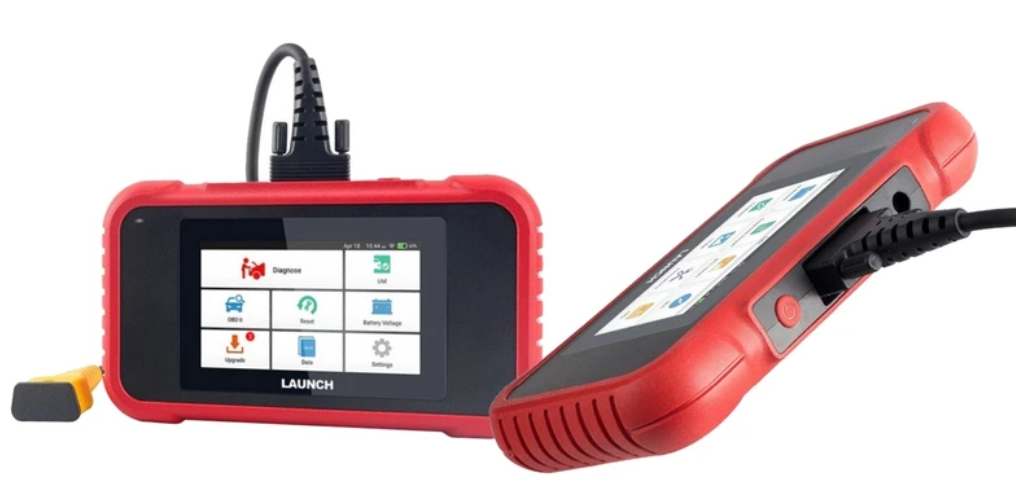
\includegraphics[width=0.63\textwidth]{Images/escaner.png}
	\vspace{0.2cm}
	
	% 3. La nota de la figura según APA 7
	\begin{flushleft}
		\footnotesize \textit{Nota.} Herramienta de diagnóstico electrónico utilizada para la lectura de códigos de falla y monitoreo de parámetros a través de la interfaz del puerto OBD-II. Tomado de \citep{OBDTester_OBD2Connector}.
	\end{flushleft}
\end{figure}

\subsection{Estructura del sistema OBD-II}% (ECU, conector, protocolos)

El sistema OBD-II está constituido por la unidad de control electrónico o ECU, el arnés de cableado, el conector de diagnóstico DLC y el protocolo de comunicación utilizado por el vehículo, que puede ser CAN, K-Line, PWM, VPW, entre otros \citep{Autoavance_OBD2, Autosoporte_OBDII, Flexihub_OBD2}. La ECU recibe señales de sensores distribuidos en el motor y, a partir del procesamiento interno, genera datos de funcionamiento, estados de actuadores y códigos de falla que pueden ser consultados a través del puerto OBD-II mediante una herramienta de diagnóstico \citep{Autoavance_OBD2, UMSA_OBDII}.

La información no sale de la ECU de forma directa hacia el escáner, sino que primero es organizada por la unidad de control en mensajes estructurados según el protocolo de comunicación del vehículo. En sistemas basados en CAN, por ejemplo, la ECU transmite y recibe tramas de datos por las líneas CAN High y CAN Low, que llegan al conector OBD-II a través del arnés eléctrico del vehículo \citep{Flexihub_OBD2, EquipoAutomotrizJAVAZ_OBD2}. En otros sistemas, la comunicación puede realizarse por una línea de datos única, como la K-Line, o por otros protocolos definidos por el fabricante \citep{Flexihub_OBD2, Autosoporte_OBDII}.

Entre la ECU y el puerto de diagnóstico intervienen principalmente el microcontrolador interno de la ECU, los circuitos de acondicionamiento de señal y los transceptores de comunicación, que adaptan los niveles eléctricos del microprocesador al bus del vehículo \citep{Autoavance_OBD2, UMSA_OBDII}. Estos transceptores permiten que la información generada dentro de la ECU sea enviada correctamente hacia el DLC sin pérdida de integridad, mientras que el escáner OBD-II actúa como elemento externo que solicita los datos y los interpreta para mostrar parámetros en tiempo real, códigos de avería y estados de sensores o actuadores \citep{Autoavance_OBD2, Autosoporte_OBDII} ver Figura \ref{fig:ecu_obd2}. De esta manera, el sistema OBD-II funciona como una interfaz estandarizada entre la electrónica interna del vehículo y el equipo de diagnóstico.

\begin{figure}[h]
	\centering
	
	% 1. El caption automático estilo APA 7 (Título arriba)
	\caption{Esquema general del flujo de información en el sistema OBD-II}
	\label{fig:ecu_obd2}
	\vspace{0.3cm}
	
	% 2. La imagen ajustada exactamente al ancho del texto
	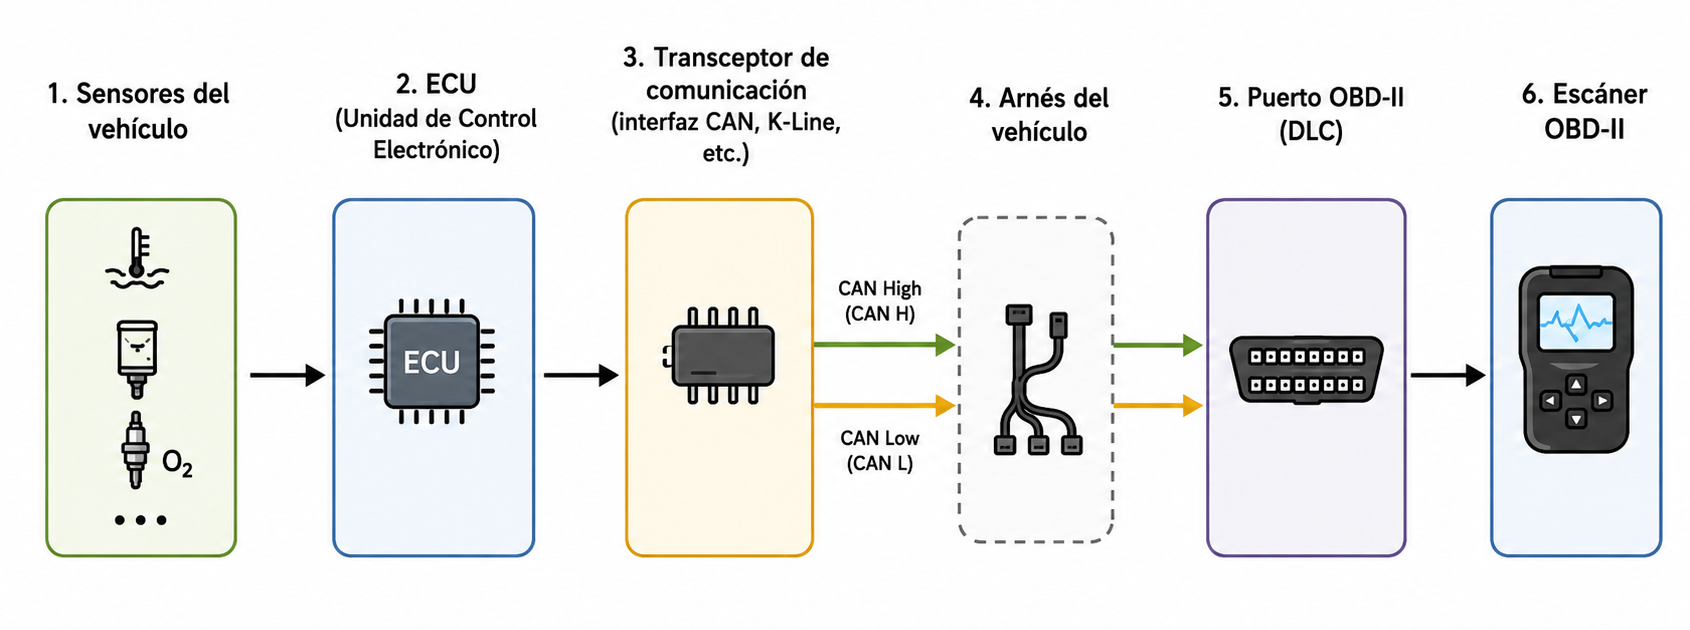
\includegraphics[width=1.0\textwidth]{Images/esquema_obd2.png}
	\vspace{0.2cm}
	
	% 3. La nota de la figura abajo alineada a la izquierda según APA 7
	\begin{flushleft}
		\footnotesize \textit{Nota.} Diagrama de bloques que describe la transmisión de datos desde la ECU y sus sensores periféricos hacia la interfaz de diagnóstico a través del bus de datos. Elaboración propia.
	\end{flushleft}
\end{figure}

\subsection{Conector OBD-II y asignación de pines}
El puerto OBD-II es una interfaz de comunicación  de 16 pines. Este puerto permite conectar dispositivos de diagnóstico, escáneres automotrices o sistemas de adquisición de datos para obtener información de las Unidades de Control Electrónico (ECU) del vehículo.  En la Figura \ref{fig:pinobd} se presenta  los pines de conexión de este puerto.

\begin{figure}[h]
	\centering
	
	% 1. El caption automático estilo APA 7 (Título conciso arriba)
	\caption{Distribución de pines del conector OBD-II}
	\label{fig:pinobd}
	\vspace{0.3cm}
	
	% 2. La imagen con su escala original
	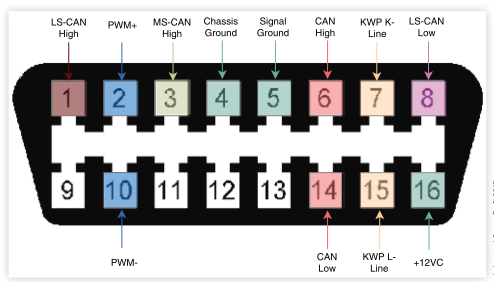
\includegraphics[width=0.5\textwidth]{Images/SEC_OBDII.png}
	\vspace{0.2cm}
	
	% 3. La nota de la figura según APA 7 (Con la descripción técnica)
	\begin{flushleft}
		\footnotesize \textit{Nota.} Configuración y asignación de los 16 pines del conector estandarizado J1962 para el diagnóstico a bordo. Tomado de \citep{OBDTester_OBD2Connector}.
	\end{flushleft}
\end{figure}

El conector OBD-II posee 16 pines, cada uno con funciones específicas dependiendo del protocolo de comunicación utilizado el detalle de cada uno de estos pines:

\begin{enumerate}
    \item LS-CAN High función específica del fabricante.
    \item Bus SAE J1850.
    \item MS-CAN High/función específica del fabricante.
    \item Tierra (chasis).
    \item Tierra de señal.
    \item CAN High (CAN alto).
    \item Línea K (ISO 9141 / ISO 14230).
    \item LS-CAN Low/función específica del fabricante.
    \item Función específica del fabricante.
    \item Bus SAE J1850/PWM.
    \item Función específica del fabricante.
    \item Función específica del fabricante.
    \item Función específica del fabricante.
    \item CAN Low.
    \item Línea L.
    \item Alimentación +12 V batería.
\end{enumerate}


En  la mayoría de los vehículos modernos, los pines 6 (CAN High) y 14 (CAN Low) son utilizados por el protocolo Controller Area Network (CAN) para la transmisión de datos entre las ECU. El puerto OBD-II puede utilizar diferentes protocolos de comunicación dependiendo del fabricante y del año del vehículo. Entre los más comunes se encuentran:
\begin{itemize}
    \item SAE J1850 PWM.
    \item SAE J1850 VPW.
    \item ISO 9141-2.
    \item ISO 14230 (KWP2000).
    \item ISO 15765-4 (CAN).
\end{itemize}

Este puerto permite solicitar información especifica mediante parámetros de identificación (Parameter ID - PIDs), los mas comunes son: 
\begin{itemize}
    \item Velocidad del vehículo.
    \item Revoluciones del motor.
    \item Temperatura del refrigerante.
    \item Posición del acelerador.
    \item Códigos de falla (DTC).
\end{itemize}
Algunas marcas permiten la visualizar una mayor cantidad de parámetros que otras, dependiendo de la cantidad de módulos con los que cuente el vehículo.
\subsection{Protocolos de comunicación}% (ISO 15765 CAN, ISO 9141, etc.)

En el sistema OBD-II existen varios protocolos de comunicación estandarizados que permiten el intercambio de información entre la ECU y el equipo de diagnóstico. En total, se consideran cinco protocolos principales de comunicación OBD-II, aunque en la práctica algunos de ellos ya han sido sustituidos por tecnologías más modernas \citep{Autoavance_OBD2, Autosoporte_OBDII, Flexihub_OBD2}.

\begin{itemize}
    \item \textbf{ISO 15765-4 CAN:} es el protocolo más utilizado en vehículos modernos. Se basa en la red CAN y utiliza las líneas CAN High y CAN Low del conector OBD-II. Se caracteriza por su alta velocidad, confiabilidad y capacidad para transmitir múltiples mensajes entre diferentes unidades de control \citep{Flexihub_OBD2, CISE_CAN}.

    \item \textbf{ISO 9141-2:} se emplea principalmente en vehículos más antiguos, especialmente de fabricantes europeos y asiáticos. Utiliza una única línea de comunicación llamada K-Line, normalmente conectada al pin 7 del conector OBD-II. Su velocidad es menor que la de CAN, pero fue muy importante en las primeras implementaciones de diagnóstico a bordo \citep{Scribd_ISO9141, Flexihub_OBD2}.

    \item \textbf{SAE J1850 PWM:} fue utilizado en algunos vehículos de origen estadounidense. Emplea una comunicación por modulación de ancho de pulso y presenta una velocidad intermedia. Aunque fue relevante en su momento, actualmente ha sido reemplazado en gran parte por CAN \citep{Autosoporte_OBDII, EquipoAutomotrizJAVAZ_OBD2}.

    \item \textbf{SAE J1850 VPW:} también fue común en vehículos de fabricantes norteamericanos. Su principal diferencia respecto a PWM es la forma de codificación de la señal, utilizando modulación por ancho de pulso variable. Tiene una arquitectura simple, pero menor capacidad que CAN \citep{Autosoporte_OBDII, EquipoAutomotrizJAVAZ_OBD2}.

    \item \textbf{ISO 14230-4 KWP2000:} conocido como \textit{Keyword Protocol 2000}, fue utilizado en varios vehículos antes de la adopción masiva de CAN. Emplea comunicación en serie sobre K-Line y permite realizar diagnósticos, lectura de datos en tiempo real y borrado de códigos de falla \citep{Autoavance_OBD2, Autosoporte_OBDII}.
\end{itemize}

En resumen como se muestra en la Tabla \ref{tab:compation}, los protocolos OBD-II evolucionaron desde soluciones más simples como K-Line y J1850 hasta el uso predominante del protocolo ISO 15765-4 CAN, que ofrece mayor velocidad, estabilidad y compatibilidad con los sistemas electrónicos actuales del vehículo \citep{Autoavance_OBD2, Flexihub_OBD2}.

\begin{table}[h]
	\centering
	% Título separado bajo norma estricta APA 7
	\captionsetup{labelformat=simple, labelsep=newline, textfont=it, labelfont=bf}
	\caption{Comparación de protocolos de comunicación OBD-II}
	\label{tab:compation}
	\vspace{0.3cm}
	
	\begin{tabularx}{\linewidth}{p{3.5cm} p{2.2cm} p{1.6cm} p{2.8cm} X}
		\toprule 
		\rowcolor[rgb]{0.851, 0.851, 0.851}
		\textbf{Protocolo} & \textbf{Medio} & \textbf{Velocidad} & \textbf{Aplicación} & \textbf{Características} \\
		\midrule 
		ISO 15765-4 CAN & CAN High / CAN Low & Alta & Vehículos modernos & Alta velocidad, confiabilidad y comunicación entre múltiples ECUs. \\
		\addlinespace
		ISO 9141-2 & K-Line & Baja & Vehículos europeos y asiáticos antiguos & Comunicación serial simple utilizada en primeras implementaciones OBD-II. \\
		\addlinespace
		SAE J1850 PWM & PWM & Media & Vehículos estadounidenses & Comunicación mediante modulación por ancho de pulso. \\
		\addlinespace
		SAE J1850 VPW & VPW & Media & Vehículos norteamericanos & Modulación por ancho de pulso variable y arquitectura simple. \\
		\addlinespace
		ISO 14230-4 KWP2000 & K-Line & Media & Vehículos previos a CAN & Permite diagnóstico, lectura de datos y borrado de códigos de falla. \\
		\bottomrule 
	\end{tabularx}
	\vspace{0.2cm}
	
	\begin{flushleft}
		\footnotesize \textit{Nota.} Elaboración propia con base en \citep{Flexihub_OBD2}, \citep{Autosoporte_OBDII} y \citep{Autoavance_OBD2}.
	\end{flushleft}
\end{table}

\subsection{Parámetros de diagnóstico (PIDs)}

Los parámetros de diagnóstico, conocidos como PIDs (\textit{Parameter IDs}), son códigos utilizados por el sistema OBD-II para solicitar y recibir información específica del funcionamiento del vehículo. Estos parámetros permiten acceder a datos en vivo provenientes de la ECU, tales como revoluciones del motor, velocidad del vehículo, temperatura del refrigerante, posición del acelerador, voltaje de sensores y otros valores relevantes para el diagnóstico \citep{Wikibooks_PIDModo01, Geotab_OBDII}.

Dentro del OBD-II, los PIDs forman parte del llamado \textit{Modo 01}, también denominado flujo de datos o datos en tiempo real. En este modo, el escáner de diagnóstico solicita a la ECU un parámetro concreto y la unidad de control responde con el valor correspondiente, que luego puede ser interpretado por el técnico para evaluar el estado de funcionamiento del motor y de los sistemas relacionados con emisiones \citep{Wikibooks_PIDModo01, OBDII_Breve}. Por ejemplo, mediante un PID es posible conocer la temperatura del motor, la carga calculada, la presión absoluta del múltiple de admisión o el estado de los sensores de oxígeno \citep{Wikibooks_PIDModo01, OBDII_Breve}.

Los PIDs no solo facilitan la lectura de variables operativas, sino que también permiten verificar si un vehículo soporta o no determinados parámetros. Esto se debe a que cada ECU responde únicamente a los PIDs que tiene implementados, lo que hace posible identificar qué información puede ser consultada en cada modelo de vehículo \citep{Wikibooks_PIDModo01, OBDII_PIDWiki}. En consecuencia, los PIDs constituyen una herramienta fundamental para el diagnóstico moderno, ya que transforman los datos internos de la ECU en información útil para el mantenimiento, la detección de fallas y el análisis de desempeño del motor \citep{Geotab_OBDII, OBDII_Breve}.

En la Tabla \ref{tab:PID} se muestra los PIDs mas utilizados y mas accesibles de ver pero de forma mas concreta se muestran en la Tabla A1 del Apéndice A.

\begin{table}[h]
	\centering
	% Título separado bajo norma estricta APA 7
	\captionsetup{labelformat=simple, labelsep=newline, textfont=it, labelfont=bf}
	\caption{PIDs OBD-II más utilizados en monitoreo vehicular}
	\label{tab:PID}
	\vspace{0.3cm}
	
	\begin{tabularx}{\linewidth}{c X c X}
		\toprule 
		\rowcolor[rgb]{0.851, 0.851, 0.851}
		\textbf{PID} & \textbf{Parámetro} & \textbf{Unidad} & \textbf{Aplicación principal} \\
		\midrule 
		0C & Velocidad del motor (RPM) & rpm & Monitoreo del rendimiento térmico y dinámico. \\
		0D & Velocidad del vehículo & km/h & Cálculo de desplazamiento y consumo de combustible. \\
		05 & Temperatura del refrigerante & °C & Supervisión térmica de las condiciones de operación. \\
		0F & Temperatura del aire de admisión & °C & Correcios en la densidad de la mezcla aire-combustible. \\
		10 & Flujo de aire másico (MAF) & g/s & Estimación absoluta de la masa de aire ingresada. \\
		11 & Posición del acelerador & \% & Detección de la carga solicitada por el conductor. \\
		04 & Carga calculada del motor & \% & Análisis de la demanda volumétrica del motor. \\
		2F & Nivel de combustible & \% & Monitoreo volumétrico de las reservas del tanque. \\
		42 & Voltaje del módulo de control & V & Diagnóstico del estado del sistema eléctrico general. \\
		03 & Códigos de falla almacenados (DTC) & --- & Diagnóstico y detección activa de averías. \\
		\bottomrule 
	\end{tabularx}
	\vspace{0.2cm}
	
	\begin{flushleft}
		\footnotesize \textit{Nota.} Elaboración propia con base en la documentación del estándar SAE J1979 y los PIDs del Modo 01.
	\end{flushleft}
\end{table}



\subsection{Importancia del OBD-II en el monitoreo del consumo de combustible}

El sistema OBD-II desempeña un papel importante en el monitoreo del consumo de combustible, ya que permite supervisar en tiempo real los parámetros que influyen directamente en la eficiencia de la combustión, como la mezcla aire-combustible, el tiempo de inyección, la señal de los sensores de oxígeno, la carga del motor y el estado del sistema de encendido \citep{MotoresUno_OBD2, Webfleet_OBD, MonitoreoOBDII}. A través de los PIDs y de los monitores internos de la ECU, el diagnóstico a bordo identifica desviaciones que pueden aumentar el consumo, como fallos de combustión, problemas en el sistema de combustible o una mala regulación de las emisiones \citep{MotoresUno_OBD2, MonitoreoOBDII}.

Cuando el sistema detecta una condición anómala, la ECU almacena códigos de falla y activa indicadores de advertencia, lo que facilita la detección temprana de problemas que afectan el rendimiento del motor y elevan el gasto de combustible \citep{Rodi_OBD2, MonitoreoOBDII}. De esta manera, el OBD-II no solo cumple una función de diagnóstico, sino que también contribuye a optimizar la operación del vehículo, reduciendo el consumo innecesario de combustible y ayudando a mantener los valores de emisiones dentro de los límites establecidos \citep{Webfleet_OBD, Autoavance_ManualOBDII}.
%-------------------------2.4----------------
\section{Red CAN}

El Controller Area Network (CAN) es un protocolo de comunicación serial diseñado para permitir la transmisión eficiente y confiable de datos entre múltiples dispositivos (módulos de sistemas específicos) electrónicos dentro de un sistema distribuido. Fue desarrollado en la década de 1980 por la empresa Robert Bosch GmbH con el objetivo de reducir la complejidad del cableado en los sistemas electrónicos de los vehículos y mejorar la comunicación entre las diferentes unidades de control electrónico.


Este protocolo permite que diferentes nodos de una red intercambien información a través de un único canal de comunicación, denominado bus, sin necesidad de una computadora central que gestione el tráfico de datos. Gracias a su arquitectura distribuida, robustez frente a interferencias electromagnéticas y capacidad de detección de errores, el bus CAN se ha convertido en uno de los estándares más utilizados en la industria automotriz y en sistemas embebidos. En la Figura ~\ref{fig:CAN_B} se presenta la conexión de diferentes módulos mediante este protocolo con dos lineas de transmisión CAN-HIGH y CAN-LOW.

\begin{figure}[h]
	\centering
	
	% 1. El caption automático estilo APA 7 (Título conciso arriba)
	\caption{Conexión de múltiples módulos mediante el protocolo CAN}
	\label{fig:CAN_B}
	\vspace{0.3cm}
	
	% 2. La imagen con su escala original
	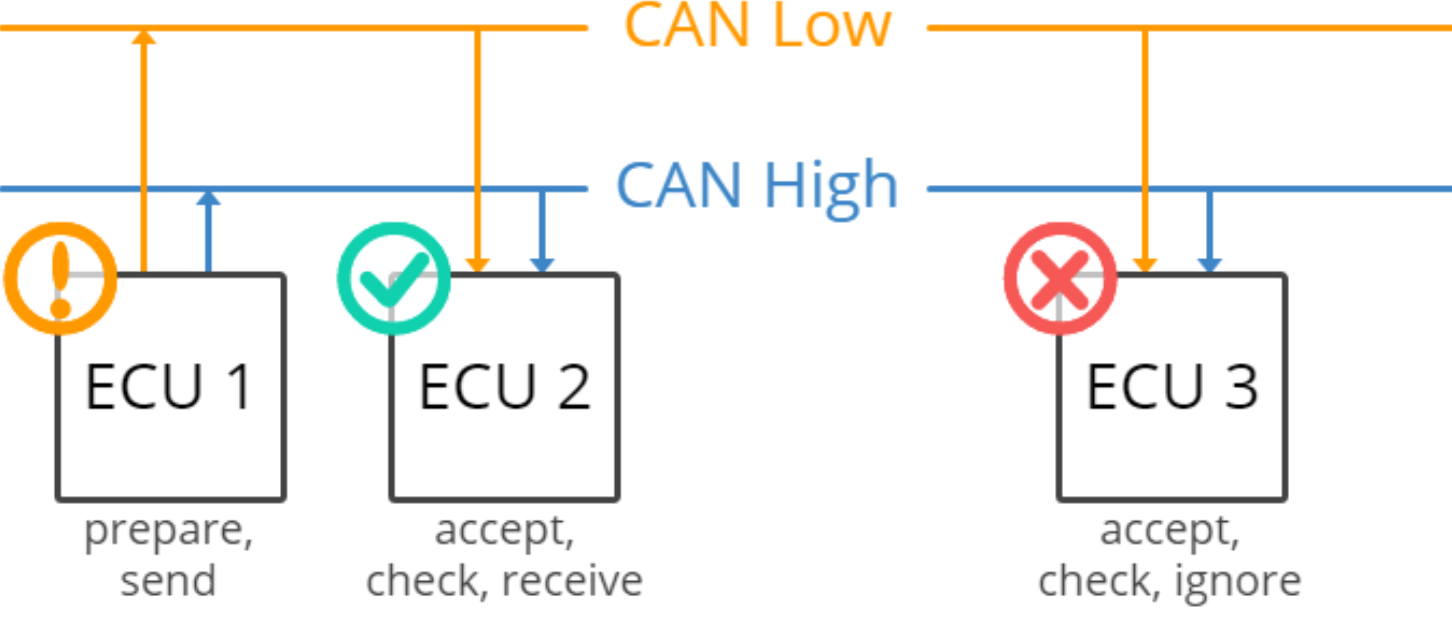
\includegraphics[width=0.5\textwidth]{Images/CAN_B.png}
	\vspace{0.2cm}
	
	% 3. La nota de la figura según APA 7 (Con la descripción técnica)
	\begin{flushleft}
		\footnotesize \textit{Nota.} Topología en bus que ilustra la interconexión en paralelo de las unidades de control electrónico compartiendo las líneas diferenciales CAN High y CAN Low. Tomado de \citep{TopeParts_EBikeProtocol}.
	\end{flushleft}
\end{figure}

\subsection{Arquitectura de la red CAN}
La implantación de este modelo de comunicaciones supuso un avance en cuanto a la cantidad de
conexiones entre dispositivos que eran necesarias para mantener todos los elementos comunicados, ya que el protocolo CAN emplea un único bus de comunicaciones, compartido por todos los dispositivos y evita la necesidad de establecer una conexión punto a punto con cada uno. Algunas de las características  que permiten a este protocolo ser adecuado para aplicaciones automotrices e industriales son:
\begin{itemize}
    \item Comunicación multi-maestro: En una red CAN no existe un nodo maestro que controle toda la comunicación. Todos los nodos conectados al bus tienen la capacidad de transmitir información cuando el canal está disponible. Esto permite una mayor flexibilidad y confiabilidad en el sistema.
    \item Comunicación basada en mensajes: A diferencia de otros protocolos de red que utilizan direcciones específicas para cada dispositivo, el bus CAN utiliza un sistema basado en identificadores de mensajes (tramas). Cada mensaje transmitido en la red contiene un identificador que indica el tipo de información que se está enviando y su nivel de prioridad. En la Figura ~\ref{fig:CAN_Frame} se presenta la estructura de datos CAN, esta cuenta de las siguientes partes:  a) Star of frame (inicio de trasmicion), b) Identifier: identificador, c) Control, d) Data (datos a transmitir), e) Cyclic Redundancy Check (detección de errores), f) Acknowledgement (confirmación) y e) End of frame (fin de trasmisión).

\begin{figure}[h]
	\centering
	
	% 1. El caption automático estilo APA 7 (Título arriba)
	\caption{Estructura de la trama de datos del protocolo CAN}
	\label{fig:CAN_Frame}
	\vspace{0.3cm}
	
	% 2. La imagen ajustada proporcionalmente al ancho del texto
	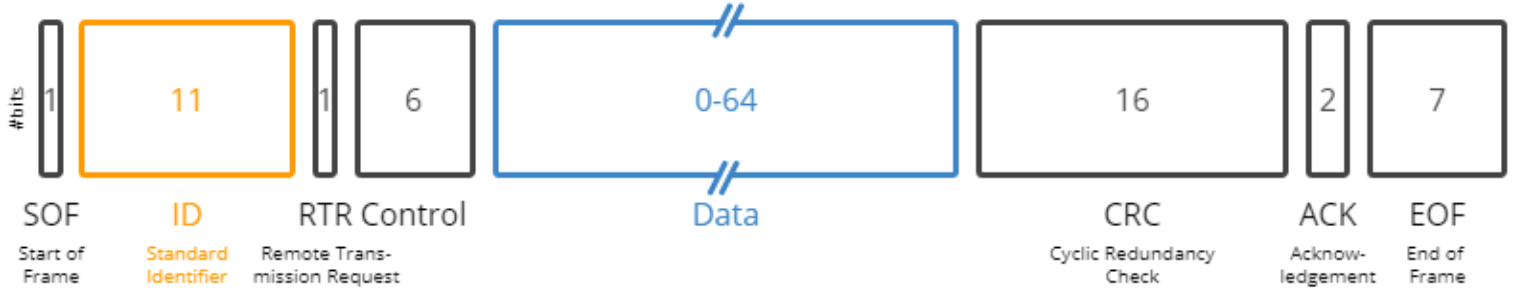
\includegraphics[width=0.9\textwidth]{Images/CAN-Frame.png}
	\vspace{0.2cm}
	
	% 3. La nota de la figura según APA 7 (Con descripción de ingeniería)
	\begin{flushleft}
		\footnotesize \textit{Nota.} Distribución de los campos de bits dentro de una trama estándar CAN, incluyendo el identificador de arbitraje, campo de control, campo de datos y el código de verificación CRC. Tomado de \citep{CarLightVision_CANBUSvsNonCANBUS}.
	\end{flushleft}
\end{figure}
    
    \item Alta inmunidad al ruido: El bus CAN utiliza una señal diferencial transmitida a través de dos líneas trenzadas denominadas CAN High y CAN Low. Esto permite reducir los efectos de interferencias electromagnéticas, lo cual es fundamental en el entorno automotriz donde existen múltiples fuentes de ruido eléctrico.
    \item Detección y manejo de errores: incluye múltiples mecanismos de detección de errores que garantizan la integridad de los datos transmitidos como: i) Verificación de redundancia cíclica (CRC); ii) Confirmación de recepción (ACK-acknowledge) y iii) Monitoreo de bits. Cuando se detecta un error, el mensaje es retransmitido automáticamente 
    
\end{itemize}

\subsection{Arquitectura física del bus CAN}
Una red CAN está compuesta por varios dispositivos denominados nodos (módulos), los cuales se conectan a un medio físico común denominado bus como se presenta en la figura ~\ref{fig:CAN_B}. Cada nodo esta compuesto principalmente por tres nodos que son:
\begin{enumerate}
    \item Microcontrolador: procesa la información del sistema y genera los datos que seran transmitidos.
    \item Controlador CAN: implementa el protocolo de comunicación CAN y gestiona la transmisión y recepción de mensajes puede estar incorporado en el microcontrolador o como un circuito externo.
    \item Transceptor CAN: convierte las señales digitales del controlador CAN en señales diferenciales que pueden transmitirse a través del bus físico.
\end{enumerate}

\section{Arquitectura física del bus CAN}
A nivel físico, el bus CAN está compuesto por una línea de comunicación diferencial formada por dos conductores. Estos dos cables transportan señales complementarias que permiten mejorar la inmunidad al ruido electromagnético. Los cables que transportan señales en protocolo CAN se identifican por ser pares trenzados como se presenta en la Figura \ref{fig:Can_Cable}.

\begin{figure}[h]
	\centering
	
	% 1. El caption automático estilo APA 7 (Título conciso arriba)
	\caption{Configuración física del cableado del protocolo CAN}
	\label{fig:Can_Cable}
	\vspace{0.3cm}
	
	% 2. La imagen con su escala original
	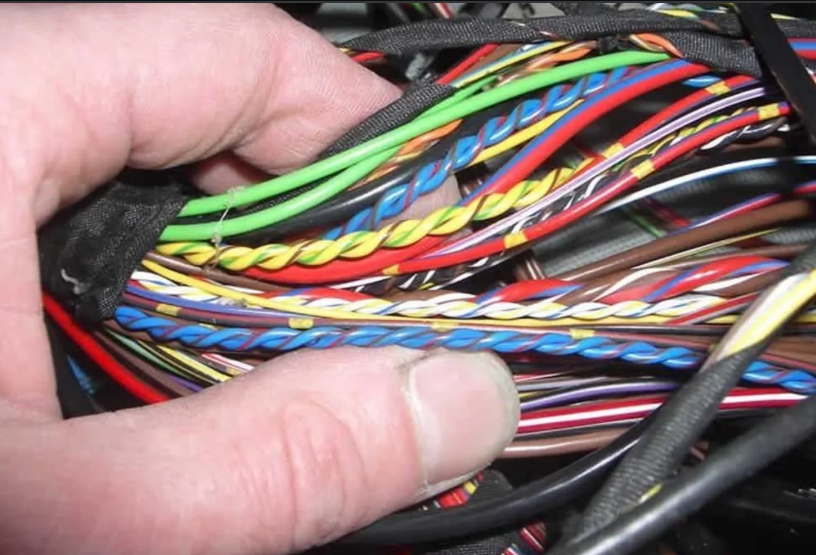
\includegraphics[width=0.6\textwidth]{Images/can cable.png}
	\vspace{0.2cm}
	
	% 3. La nota de la figura según APA 7 (Con descripción técnica)
	\begin{flushleft}
		\footnotesize \textit{Nota.} Disposición física de las líneas diferenciales de comunicación mediante par trenzado, diseñada para mitigar el ruido electromagnético en el entorno automotriz. Tomado de \citep{CarLightVision_CANBUSvsNonCANBUS}.
	\end{flushleft}
\end{figure}

El bus puede encontrarse en modo recesivo, con ambos cables con el mismo nivel de tensión o en modo dominante. En estado recesivo (inactivo), ambas líneas están cerca de 2,5V. En estado dominante (activo), CAN-H sube a 3,5V y CAN-L baja a 1,5V,Este modo de comunicación tiene como objetivo proporcionar una mayor protección frente a interferencias electromagnéticas. Esta protección viene dada, debido a que la lectura de los bits se basa en la diferencia de voltaje entre los dos cables trenzados, por lo que en caso de verse sometidas a la misma influencia electromagnética, a pesar de la variación señal en los cables, la diferencia de voltaje entre ellos se mantiene constante.

 En la Figura ~\ref{fig:Can_Volt} se presenta los niveles de voltaje de este protocolo. En el bus, los bits dominantes equivalen al nivel lógico "0", y los bits recesivos al valor lógico "1".
 
\begin{figure}[h]
	\centering
	
	% 1. El caption automático estilo APA 7 (Título conciso arriba)
	\caption{Niveles de voltaje diferencial en el bus CAN}
	\label{fig:Can_Volt}
	\vspace{0.3cm}
	
	% 2. La imagen con su escala original
	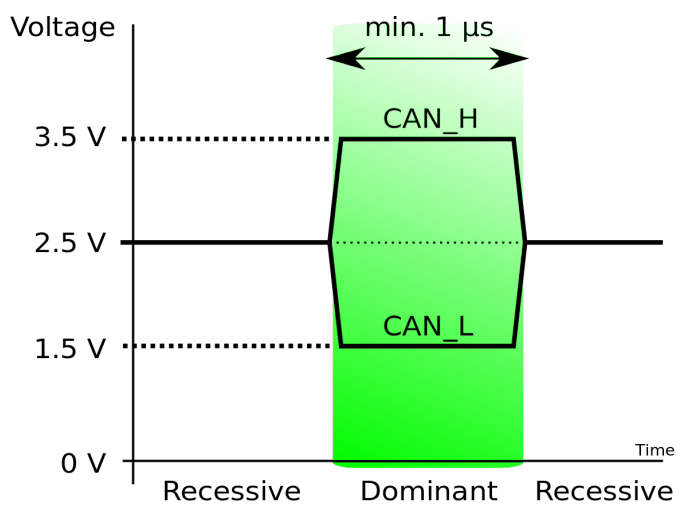
\includegraphics[width=0.6\textwidth]{Images/Can_Volt.png}
	\vspace{0.2cm}
	
	% 3. La nota de la figura según APA 7 (Con descripción técnica)
	\begin{flushleft}
		\footnotesize \textit{Nota.} Comportamiento eléctrico de las señales CAN High y CAN Low durante los estados lógicos dominante y recesivo para la transmisión física de datos. Tomado de \citep{Jidoshaseibishi_19}.
	\end{flushleft}
\end{figure}
    
\subsection{Topología del bus CAN}
Posee una topología en forma de bus, en la que únicamente son necesarios dos cables trenzados y todos los nodos se conectan a un mismo cable principal. En los extremos del bus se colocan resistencias de terminación, generalmente de 120 ohmios, con el objetivo de evitar reflexiones de señal y garantizar la estabilidad de la comunicación. \citep{Lifeder_BusTopology,IndustrialMonitorDirect_CANTermination}

La longitud máxima del bus depende de la velocidad de transmisión utilizada. Tabla \ref{bus_length} se presenta la velocidad, longitud y tiempo de transmisión  mediante este protocolo de comunicación a diferentes distancias. 

\begin{table}[h]
	\centering
	% Título separado bajo norma estricta APA 7
	\captionsetup{labelformat=simple, labelsep=newline, textfont=it, labelfont=bf}
	\caption{Relación entre longitud del bus, velocidad y tiempo máximo de transmisión}
	\label{bus_length}
	\vspace{0.3cm}
	
	% Usamos tabularx equilibrando las tres columnas uniformemente
	\begin{tabularx}{\linewidth}{X X X}
		\toprule % Línea superior APA 7
		\rowcolor[rgb]{0.851, 0.851, 0.851}
		\textbf{Longitud del bus} & \textbf{Velocidad (bits/s)} & \textbf{Tiempo máximo de transmisión} \\
		\midrule % Línea divisoria de encabezado APA 7
		Hasta 25 m & 1 Mbit/s & 129 $\mu$s \\
		\addlinespace
		Hasta 100 m & 500 Kbit/s & 258 $\mu$s \\
		\addlinespace
		Hasta 500 m & 125 Kbit/s & 1032 $\mu$s \\
		\addlinespace
		Hasta 1000 m & 50 Kbit/s & 2580 $\mu$s \\
		\bottomrule % Línea inferior de cierre APA 7
	\end{tabularx}
	\vspace{0.2cm}
	
	\begin{flushleft}
		\footnotesize \textit{Nota.} Elaboración propia.
	\end{flushleft}
\end{table}



\subsection{Tramas del protocolo CAN}
El protocolo CAN contempla diferentes formatos de tramas, cada una orientada a un propósito específico dentro del funcionamiento del protocolo en la figura ~\ref{fig:CAN_Frame} se presentan las partes mas importantes  que son:
\begin{itemize}
    \item Tramas de datos: utilizadas para el paso de información entre nodos, que puede ser  enviada y recibida por uno o varios de ellos.
    \item Tramas de error:  utilizadas cuando algún nodo de la red detecta un error en alguno de los mensajes transmitidos por otros nodos de la red conectada.
    \item Tramas de petición remota: utilizadas para solicitar el envío de información a otro nodo. Se envía una trama con el identificador (id) del nodo del que se requiere el envío de información, éste recibe la trama y devuelve la información con los datos solicitados. 
    \item Tramas de sobrecarga: utilizadas para detectar errores de sobre carga.  Es enviada por un nodo cuando éste está sobrecargado, provoca un retardo en la comunicación.
\end{itemize}

Cuando el bus esta en retardo no existe flujo de tramas y el bus se mantiene en estado recesivo. Cuando el bus requiere enviar mas de una trama estas deben estar separadas por una secuencia predeterminada (intertrama) que esta compuesta por tres bits recesivos.

Los datos enviados por este protocolo son de hasta 8 bytes. En la figigura \ref{fig:Frame} se presenta el formato de esta trama requiere 1 bit  para el inicio de la secuencia se cuenta empleado para la sincronización con el resto de la secuencia. Posteriormente se encuentra el identificador de 11 bits. Conociendo los identificadores de todas las tramas que intentan ser transmitidas, se puede establecer de manera determinista el orden en el que son transmitidas. Se puede establecer un orden para priorizar algunas tramas sobre otras por ejemplo: una trama CAN con identificador más bajo (mayor número de bits dominantes en las primeras posiciones) tiene más prioridad que una trama con identificador más alto. 

Para el campo de control los dos bits iniciales están reservados para un uso futuro, y posteriormente
se encuentran cuatro bits, que definen el tamaño del campo de datos de la trama que se encuentra a
continuación. La parte de la trama coloreada en rojo en la Figura \ref{fig:Frame} es la de datos que puede abarcar hasta 8 bytes. El campo CRC (Código de redundancia cíclica), se encarga de asegurar la integridad de los datos enviados esta cuenta con 15 bit y un bit adicional un bit recesivo como delimitador. La trama continua con 2 bits de confirmación o reconocimiento ACK (acknowledge) y finalmente se envían los bits de fin de trama EOF(end of frame) que contiene 7 bits. Adicionalmente la trama debe contener tres bits de espaciado al final de trama.

\begin{figure}[h]
	\centering
	
	% 1. El caption automático estilo APA 7 (Título conciso arriba)
	\caption{Campos constitutivos del formato de trama de datos CAN}
	\label{fig:Frame}
	\vspace{0.3cm}
	
	% 2. La imagen ajustada proporcionalmente al ancho del texto
	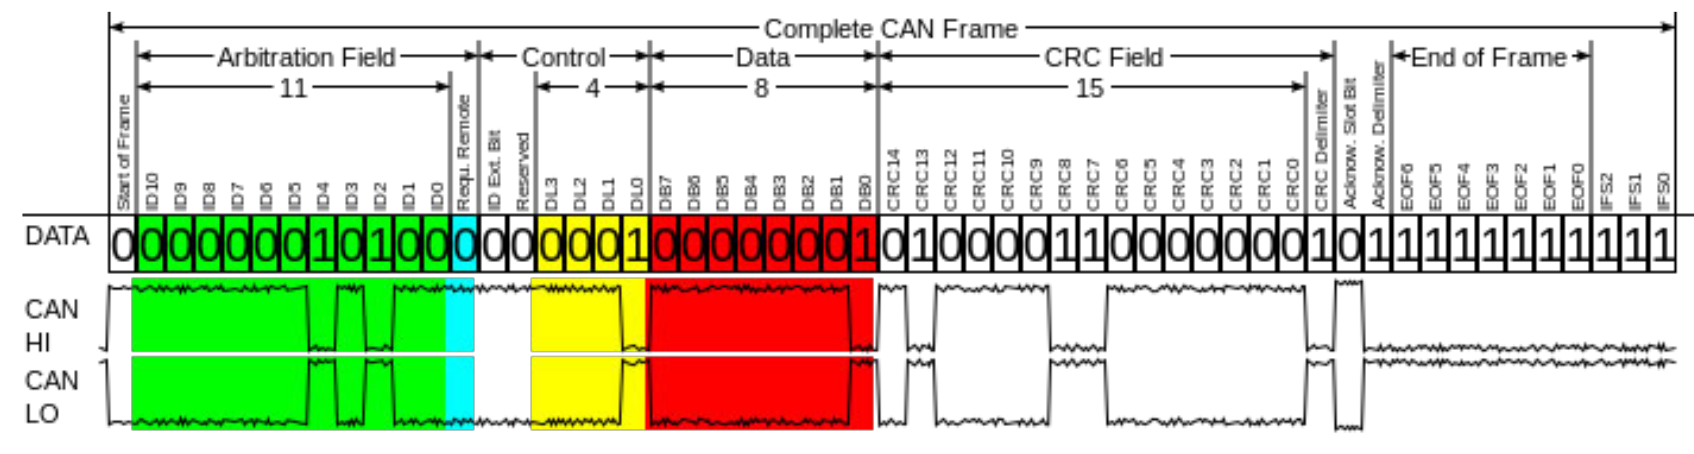
\includegraphics[width=0.9\textwidth]{Images/Frame.png}
	\vspace{0.2cm}
	
	% 3. La nota de la figura según APA 7 (Con descripción técnica)
	\begin{flushleft}
		\footnotesize \textit{Nota.} Segmentación detallada del formato de la trama estándar, especificando la longitud y función de los bits de inicio, arbitraje, control, datos, CRC, ACK y fin de trama (*EOF*). Tomado de \citep{Jeong_Ch7VehicleNetwork}.
	\end{flushleft}
\end{figure} 

\subsection{Errores en trama de datos}

El protocolo CAN posee una norma de relleno de bits en las tramas, que consiste en que cada secuencia de cinco bits con el mismo valor, se introduce un bit de valor inverso. Esto provoca que el formato de las tramas de error incumplan esta norma y puedan ser detectadas sobre las tramas de datos. Estas tramas de error pueden ser generadas por cualquier nodo que detecte un error en la comunicación. Se componen de dos campos. Se compone de dos campos primero se encuentra el indicador de error, o error flag, cuyo formato depende el tipo de nodo que haya detectado el error. En la Figura \ref{fig:Errorp}, se describen las partes de esta trama. 


\begin{figure}[h]
	\centering
	
	% 1. El caption automático estilo APA 7 (Título conciso arriba)
	\caption{Estructura de una trama de error en el protocolo CAN}
	\label{fig:Errorp}
	\vspace{0.3cm}
	
	% 2. La imagen ajustada proporcionalmente al ancho del texto
	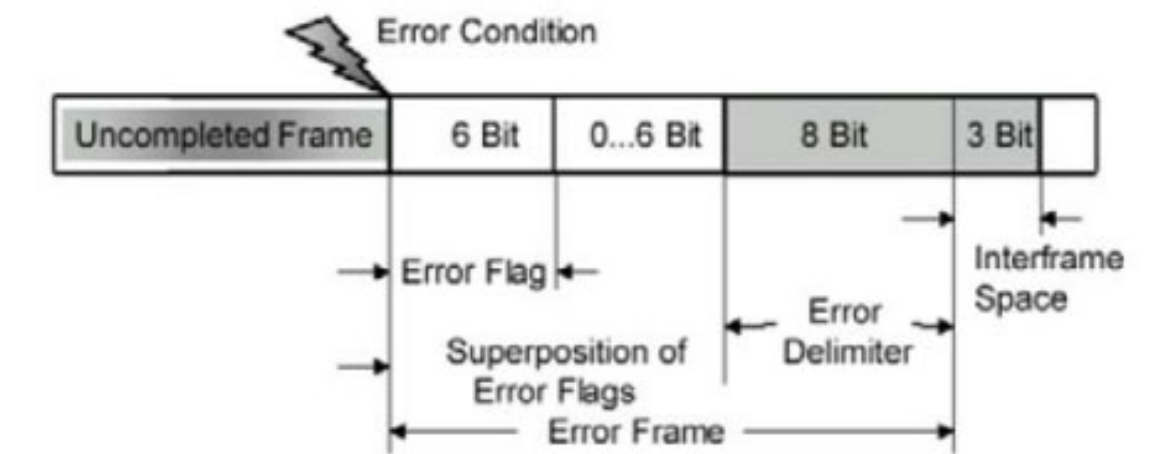
\includegraphics[width=0.8\textwidth]{Images/Error.png}
	\vspace{0.2cm}
	
	% 3. La nota de la figura según APA 7 (Con descripción técnica)
	\begin{flushleft}
		\footnotesize \textit{Nota.} Configuración de los campos de la trama de error, detallando los bits de delimitación y la secuencia de banderas de error activas o pasivas utilizadas para la gestión de fallas en el bus. Tomado de \citep{NCKU_EmbeddedWiki}.
	\end{flushleft}
\end{figure}

Para evitar que un nodo con errores condicione el funcionamiento de la red o pueda provocar fallos o saturaciones, el protocolo dispone de medidas para desconectar de la red este tipo de nodos. Los nodos pueden estar en tres tipos de estado diferente que son:
\begin{itemize}
    \item Error activo: El nodo puede enviar mensajes y tramas de error normalmente. Es el estado normal.
    \item Error pasivo: El nodo cambia el formato de sus tramas de error, enviando 12 bits recesivos. De este modo, el resto de nodos no son capaces de detectarlas y no ralentiza las comunicaciones.
    \item Bus off o Anulado: El nodo se auto-desconecta del bus, se deshabilita su transceptor y no participa en la comunicación.
\end{itemize}

Cuando un nodo se desconecta de la red, se resetea, configura y se conecta de nuevo a la red, pero no podrá comenzar a transmitir de nuevo hasta no haber recibido 128 secuencias de 11 bits recesivos sin errores en el bus.
\subsection{Red CAN en vehículos}

La red CAN (\textit{Controller Area Network}) es uno de los protocolos de comunicación más utilizados en vehículos modernos debido a su capacidad para permitir la comunicación entre múltiples unidades de control electrónico (ECU) mediante un bus compartido. A través de esta red, distintos módulos del vehículo intercambian información relacionada con el motor, transmisión, frenos, sistemas de seguridad y otros subsistemas electrónicos \citep{Flexihub_OBD2, CISE_CAN}. 

En los sistemas OBD-II modernos, especialmente aquellos basados en el protocolo ISO 15765-4, la comunicación de diagnóstico se realiza sobre la red CAN utilizando identificadores específicos para solicitudes y respuestas. Generalmente, las herramientas de diagnóstico envían solicitudes mediante el identificador funcional 0x7DF, mientras que las ECU responden utilizando identificadores comprendidos entre 0x7E8 y 0x7EF \citep{Flexihub_OBD2}. Mediante este mecanismo es posible consultar parámetros estandarizados conocidos como PIDs (\textit{Parameter IDs}), los cuales permiten obtener datos como velocidad del vehículo, revoluciones del motor, temperatura del refrigerante o flujo de aire del motor.

Sin embargo, además de los PIDs normalizados definidos por el estándar OBD-II, los fabricantes implementan protocolos CAN propietarios para la comunicación interna entre las ECU del vehículo. Estos mensajes no se encuentran documentados públicamente y varían dependiendo de la marca, modelo y año del vehículo. Debido a ello, gran parte de la información transmitida en la red CAN no puede ser interpretada directamente sin realizar procesos de ingeniería inversa (\textit{reverse engineering}) \citep{Flexihub_OBD2, CAN_D_2020}.

La ingeniería inversa sobre redes CAN consiste en capturar y analizar las tramas transmitidas por las ECU con el objetivo de identificar qué mensajes corresponden a determinados parámetros del vehículo. Para ello, normalmente se registra el tráfico CAN mientras se modifica una variable específica del vehículo, por ejemplo acelerar, activar luces o mover el volante. Posteriormente se analizan los identificadores CAN y los bytes de datos que presentan variaciones relacionadas con dicha acción \citep{reddit_CAN_reverse, embedded_CAN_reverse}. 

Un aspecto importante en el análisis de tramas CAN es la interpretación de los datos binarios transmitidos por las ECU. Cada mensaje CAN contiene una secuencia de bytes que representan información específica del vehículo, la cual debe convertirse desde formato hexadecimal o binario a valores numéricos comprensibles conocidos como DBC \citep{Flexihub_OBD2}. 

\subsection{Archivo DBC CAN}

Un archivo CAN DBC (CAN Database) es un archivo de texto que contiene la información necesaria para decodificar los datos sin procesar transmitidos por la red CAN y convertirlos en valores físicos interpretables. Este tipo de archivo define la estructura de los mensajes y de las señales asociadas, permitiendo establecer cómo debe leerse cada dato dentro de una trama CAN.

La Figura \ref{fig:dbc_sintaxis} presenta la estructura básica de un mensaje y de una señal dentro de un archivo DBC. Este tipo de archivo se utiliza para describir la forma en que los datos transmitidos a través de la red CAN deben ser interpretados, permitiendo asociar los valores binarios con variables físicas de interés.

\begin{figure}[htbp]
	\centering
	
	% 1. El caption automático estilo APA 7 (Título arriba)
	\caption{Sintaxis básica de un mensaje y una señal en un archivo DBC}
	\label{fig:dbc_sintaxis}
	\vspace{0.3cm}
	
	% 2. La imagen ajustada proporcionalmente al ancho del texto
	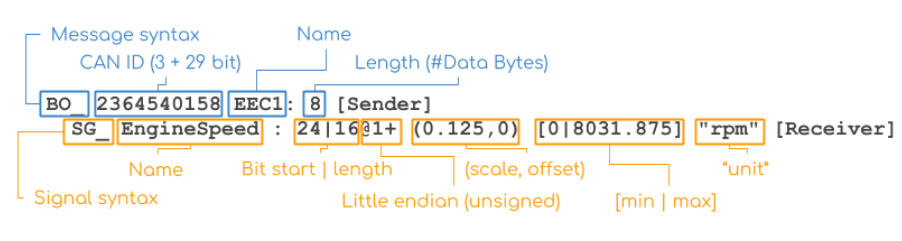
\includegraphics[width=0.9\textwidth]{Images/BDC.png}
	\vspace{0.2cm}
	
	% 3. La nota de la figura según APA 7 (Con descripción técnica)
	\begin{flushleft}
		\footnotesize \textit{Nota.} Estructura de codificación en bases de datos CAN (*.dbc*), donde se definen los identificadores de los mensajes (BO\_), los nombres de las señales (SG\_), el orden de los bits (*endianness*), el factor de escala y el offset de conversión. Elaboración propia.
	\end{flushleft}
\end{figure}

En la parte superior de la figura se muestra la sintaxis correspondiente a un mensaje, identificada con el prefijo \texttt{BO\_}. En esta definición se incluye el identificador CAN, el nombre del mensaje, la longitud expresada en número de bytes de datos y el nodo transmisor. Estos elementos permiten describir de manera ordenada cada trama que circula por el bus CAN.

En la parte inferior se presenta la sintaxis de una señal, indicada mediante el prefijo \texttt{SG\_}. En este caso, se especifica el nombre de la señal, la posición inicial del bit, la longitud de la señal, el orden de bytes, el tipo de dato, el factor de escala, el desplazamiento, el rango físico, la unidad de medida y el nodo receptor. La combinación de estos parámetros define cómo debe interpretarse cada señal contenida dentro de un mensaje.

Por ejemplo, en la señal mostrada en la figura, \texttt{EngineSpeed} corresponde al nombre de la señal; \texttt{24|16} indica que la señal inicia en el bit 24 y tiene una longitud de 16 bits; \texttt{@1+} señala una codificación little-endian y un dato sin signo; \texttt{(0.125,0)} representa el factor de escala y el desplazamiento; \texttt{[0|8031.875]} define el rango físico de la señal, y \texttt{rpm} establece la unidad de medida.

En este sentido, el archivo DBC funciona como una guía de decodificación que permite transformar los datos crudos del bus CAN en magnitudes físicas comprensibles, tales como velocidad, régimen del motor, temperatura o presión. Por ello, constituye una herramienta fundamental en aplicaciones de diagnóstico automotriz, monitoreo de variables vehiculares, telemetría e ingeniería inversa de redes CAN.

Un ejemplo simplificado de sintaxis DBC para la velocidad del vehículo es el siguiente:\\

\begin{verbatim}
	BO_ 2024 OBD2: 8 Vector__XXX
	SG_ VehicleSpeed : 0|8@1+ (1,0) [0|255] "km/h" Vector__XXX
\end{verbatim}

En este ejemplo, \texttt{VehicleSpeed} es el nombre de la señal, \texttt{0|8} indica que la señal comienza en el bit 0 y tiene una longitud de 8 bits, \texttt{@1+} señala que usa little-endian y que es no firmada, \texttt{(1,0)} corresponde al factor de escala y al desplazamiento, \texttt{[0|255]} define el rango físico permitido, \texttt{"km/h"} representa la unidad y \texttt{Vector\_\_XXX} actúa como nodo genérico.

Por ejemplo, una trama CAN correspondiente a una respuesta OBD-II puede representarse de la siguiente manera:

\begin{center}
	\texttt{7E8 03 41 0D 37 FF FF FF FF}
\end{center}

En esta trama, \texttt{7E8} corresponde al identificador de respuesta de la ECU, \texttt{41} indica una respuesta positiva al modo de diagnóstico 01, \texttt{0D} representa el PID de velocidad del vehículo y \texttt{37} contiene el valor de la señal. Al convertir \texttt{37} de hexadecimal a decimal se obtiene 55, por lo que la velocidad interpretada es de \texttt{55 km/h}.

De esta manera, los archivos DBC permiten transformar datos CAN sin procesar en variables físicas útiles para aplicaciones de monitoreo vehicular, diagnóstico automotriz, telemetría e ingeniería inversa de redes CAN.

%-------------------------2.5----------------

